\section{Aufbau und Durchführung}
\label{sec:Durchführung}
\subsection{Messreihe zur Bestimmung der Zeitkonstanten mit Hilfe des Entladevorgangs}
Der Versuch wird wie in Abbildung \ref{fig:aufbauent} aufgebaut. Dazu werden ein Kondensator mit der Kapazität $C$ und ein Widerstand mit dem
Ohm'schen Widerstand R an einen Spannungsgenerator und ein Oszilloskop angeschlossen. Es wird eine Rechteckspannung mit Hilfe des Generators erzeugt.
Die Rechteckfrequenz und die Einstellungen am Oszilloskop werden so gewählt, dass sich $U(t)$ um den Faktor 5 bis 10 ändert.
Es werden 15 bis 20 Messwerte von $U(t)$ und den dazugehörigen Zeiten abgelesen.
\begin{figure}
    \centering
    \caption{Aufbau zur Bestimmung der Zeitkonstante eines Entladevorgangs} 
    \label{fig:aufbauent}
    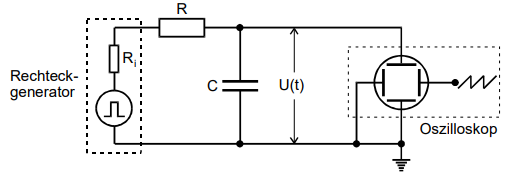
\includegraphics[width = 0.5\textwidth]{pics/aufbauent.png}
\end{figure}
\subsection{Messreihe zur Bestimmung von Spannungsamplituden}
Der Aufbau für die Messreihe ist Identisch zu dem Vorherigen. Statt einer Rechteckspannung wird nun eine Sinusspannung erzeugt, 
bei der sich die Frequenz anpassen lässt. In der Durchführung wird nun die Frequenz am Sinusgenerator logarithmisch erhöht und es wird am Oszilloskop die 
Amplitude $A(\omega)$ gemessen. Dies wird 15 bis 20 mal wiederholt.
\subsection{Messreihe zur Bestimmung der Phasenverschiebung}
\label{subsec:Phase}
In der dritten Messreihe soll die Phasenverschiebung ermittelt werden. Dazu wird der Versuch wie in Abbildung \ref{fig:aufbauphi} aufgebaut.
Es wird wieder eine Sinusspannung angelegt und die Frequenzen werden logarithmisch erhöht.
Dadurch lassen sich die Phasenverschiebungen in Abhängigkeit von $\omega$ mit
\begin{equation}
    \varphi=\frac{a}{b} \, 2 \pi \label{eqn:phiab}
\end{equation}
berechnen, dabei werden die Werte a und b wie in \ref{fig:wertphi} abgelesen.
Mit der Phasenverschiebung $\varphi$, lässt sich die Zeitkonstante bestimmen. Dazu kann die Gleichung
\begin{equation}
    \label{eqn:ficken}
    \varphi (\omega)=\arctan (-\omega RC)
\end{equation}
verwendet werden.
\begin{figure}
    \centering
    \caption{Aufbau zur Bestimmung der Phasenverschiebung} 
    \label{fig:aufbauphi}
    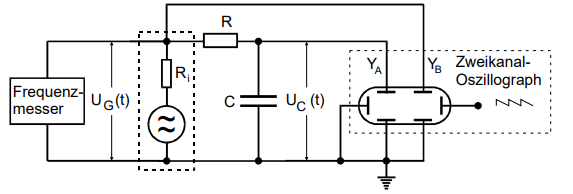
\includegraphics[width = 0.5\textwidth]{pics/phasenverschiebung.png}
\end{figure}
\begin{figure}
    \centering
    \caption{Skizze zur Bestimmung der Phasenverschiebung} 
    \label{fig:wertphi}
    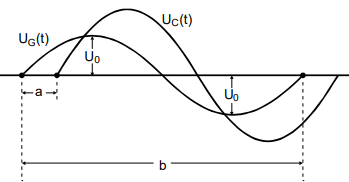
\includegraphics[width = 0.5\textwidth]{pics/werteabl.png}
\end{figure}
\subsection{Messreihe zur Integratorfähigkeit des RC-Kreises}
Für diese Messreihe kann der Versuchsaufbau aus \ref{subsec:Phase} übernommen werden.
Auf dem Oszilloskop sind die Spannungsverläufe $U(t)$ des Generators und die integrierte Spannung $U_\text{C}(t)$ zu erkennen.
Am Generator werden nacheinander eine Rechteckspannung, eine Dreieckspannung und zuletzt eine Sinusspannung erzeugt.
Dadurch entstehen drei verschiedene Bilder der zwei Spannungsverläufe. Diese werden dann abfotografiert. 